% Unofficial University of Lethbridge Poster template.
% A fork of unofficial University of Alberta Poster template: 
% which is a fork of Yale template: https://www.overleaf.com/latex/templates/yale-poster-template/rjpgqfgvsjcv
% which is a fork of the UMich template https://www.overleaf.com/latex/templates/university-of-michigan-umich-poster-template/xpnqzzxwbjzc
% which is fork of the MSU template https://www.overleaf.com/latex/templates/an-unofficial-poster-template-for-michigan-state-university/wnymbgpxnnwd
% which is a fork of https://www.overleaf.com/latex/templates/an-unofficial-poster-template-for-new-york-university/krgqtqmzdqhg
% which is a fork of https://github.com/anishathalye/gemini
% also refer to https://github.com/k4rtik/uchicago-poster



\documentclass[final]{beamer}

% ====================
% Packages
% ====================

\usepackage[T1]{fontenc}
 \usepackage[utf8]{luainputenc}
\usepackage{lmodern}
\usepackage[size=a1, orientation=landscape, scale=1.43]{beamerposter}
\usetheme{gemini}
\usecolortheme{msu}
\usepackage{graphicx}
\usepackage{booktabs}
\usepackage{tikz}
\usepackage{pgfplots}
\pgfplotsset{compat=1.14}
\usepackage{anyfontsize}

\usepackage{arev}
\usepackage[T1]{fontenc}

% ====================
% Lengths
% ====================

% If you have N columns, choose \sepwidth and \colwidth such that
% (N+1)*\sepwidth + N*\colwidth = \paperwidth
\newlength{\sepwidth}
\newlength{\colwidth}
\setlength{\sepwidth}{0.01\paperwidth}
\setlength{\colwidth}{0.48\paperwidth}

\newcommand{\separatorcolumn}{\begin{column}{\sepwidth}\end{column}}


% ====================
% Title
% ====================

\title{Implementation of a Basic Blockchain with PoW and Merkle Patricia Tries}

\author{Joel González Jiménez}

\institute[shortinst]{Master in Innovation and Research in Informatics (MIRI) | Computer Networks \& Distributed Systems }


% use this to include logos on the left and/or right side of the header:
% \logoright{
\includegraphics[height=8cm]{logos/UofL_Landscape_RGB_FullColourRev.png}}


\begin{document}


\begin{frame}[t]
\begin{columns}[t]
\separatorcolumn

\begin{column}{\colwidth}

	\vspace{-1em}
  \begin{block}{\LARGE 1. Introduction}
  	
    Blockchain research is continually driving new functionalities and optimizations. As a result, modern blockchains look vastly different from the beginning. 
    
    This project is a hands-on implementation of a blockchain designed to isolate and study the core focusing on:
    
    \begin{itemize}
    	\item \textbf{Consensus mechanism} (PoW)
    	\item \textbf{Merkle Patricia Trie} (MPT)
    \end{itemize}
    
  \end{block}
  \vspace{-1em}
  \begin{block}{\LARGE 2. Capabilities}
  	
%  	\begin{itemize}
%  		\item \textbf{Block immutability}
%  		\item \textbf{Lightweight Verification (MPT Proofs)}
%  		\item \textbf{Persistant Storage}
%  		\item \textbf{Debuging tools and tests}
%  	\end{itemize}

	\begin{itemize}
		\item \textbf{Cryptographic Immutability:} Ensuring integrity via sequential SHA-256 block-hashing and Proof-of-Work consensus.
		\item \textbf{Lightweight Verification:} Utilizing Merkle Patricia Trie (MPT) cryptographic proofs $O(\log n)$.
		\item \textbf{Persistent State Storage:} Implementing data-store layer to preserve the blockchain across experimental runs.
		\item \textbf{Debuging tools and tests:} Integrated tools for analyzing the content of blocks in the blockchain and growth.
	\end{itemize}

  	
  \end{block}
  \vspace{-1em}
  \begin{block}{\LARGE 3. Merkle Patricia Trie (MPT)}
  	\vspace{1em}
  	\begin{minipage}[c]{0.4\linewidth}
  		
		\begin{tabular}{ll}
			\toprule
			\textbf{Key} & \textbf{Value} \\
			\midrule
			0xA7333 & DUCK \\
			0xA73EB & PIE \\
			\bottomrule
		\end{tabular} \\
		\vspace{1em}
		
		Differences from standard MPT:
		\begin{itemize}
			\item Use of GOB encoder instead of RLP.
			\item Branch node does not contain value because all keys have equal length.
			\item The key of a value (path), is the hash of value itself.
			\item The values stored are strings transformed to bytes
		\end{itemize}
	\end{minipage}% 
	\hfill
  	\begin{minipage}[c]{0.55\linewidth}
	  	\begin{center}
	  		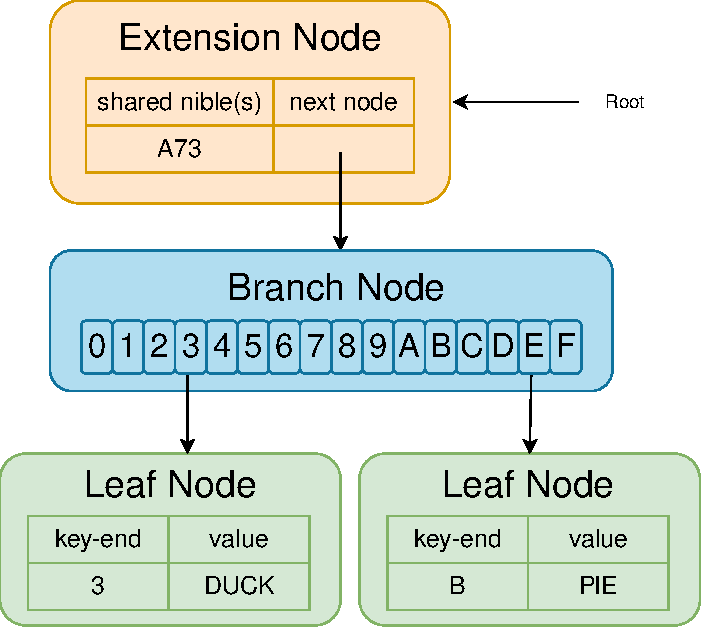
\includegraphics[width=1\linewidth]{figures/MPT.pdf}
	  		\centering
	  	\end{center}
	\end{minipage}
  	
  \end{block}

\end{column}

\separatorcolumn

\begin{column}{\colwidth}
	\vspace{-1em}
	\begin{block}{\LARGE 4. Consensus (PoW)}
		
		\Large
		\vspace{-1em}
		\begin{equation*}
			\text{SHA256}(\text{BlockData} \parallel \text{Nonce}) < \text{Target}
		\end{equation*}
		\vspace{-1em}
		\begin{equation*}
			\text{Target} = 1 << (\text{HashLength} - \text{Difficulty})
		\end{equation*}
		
		\begin{center}
			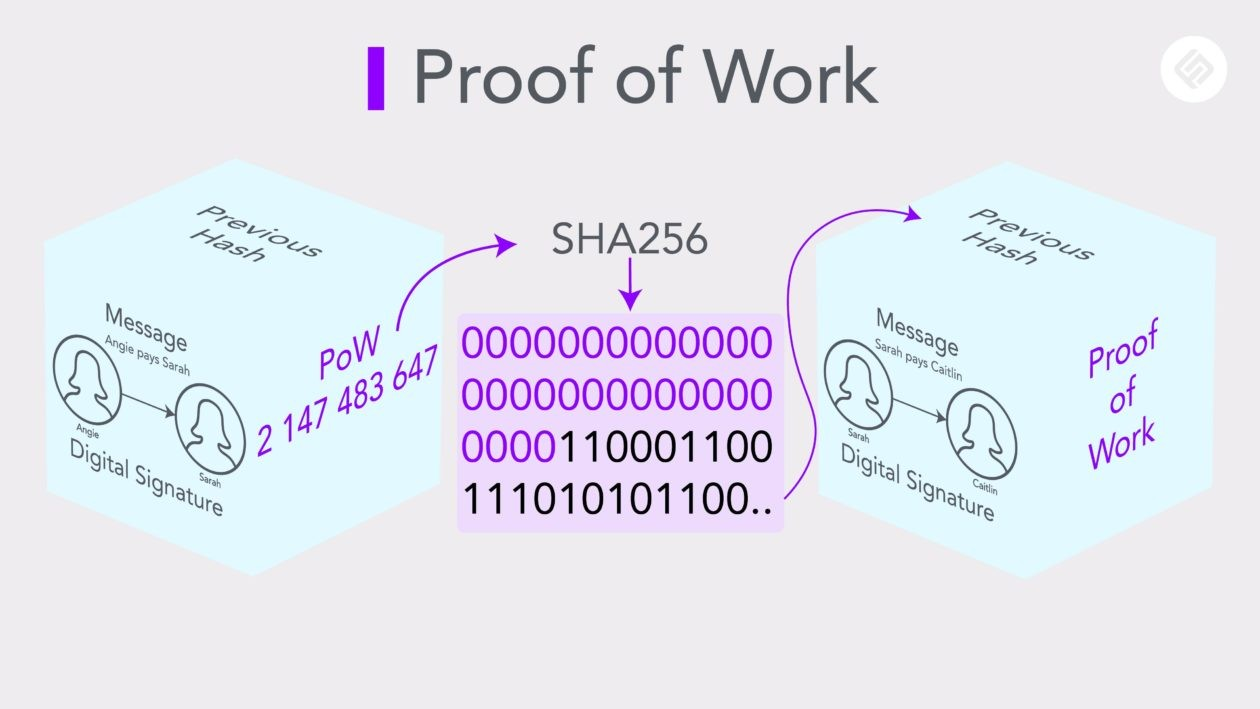
\includegraphics[width=0.6\linewidth]{figures/PoW.jpg}
			\centering
			\setlength{\fboxsep}{1em}
		\end{center}
	\end{block}
	\vspace{-1em}
	\begin{block}{\LARGE 5. Class diagram}
		Architectural design prioritizes modularity and enforces an acyclic dependency graph among classes and defines responsibilities for each component.

		\begin{center}
			
\includegraphics[width=1\linewidth]{figures/simplest_diagram.png}
			%    	\includesvg{figures/complete_diagram.svg}
			\centering
			\setlength{\fboxsep}{1em}
		\end{center}
		
	\end{block}

\end{column}

\separatorcolumn
\end{columns}
\end{frame}

\end{document}
